\section{Introduction}
\label{sec:introduction}

Robot teams increasingly rely on learned models that predict how the world, the
task, and other robots will evolve.  Most deployments run these models on shared
infrastructure and stream the results back to the robots.  Running prediction on
board instead, next to the controller that consumes it, shortens the path
between an observation and the decision that depends on it.  It also changes
which component owns the result and how far the result travels before it is
used.

These notes follow a command through a multi-robot team, from the operator's
intent to physical motion, and ask what happens to a prediction along the way.
Classical coordination already separates task allocation, conflict resolution,
and motion \cite{gerkey2004mrta,choi2009cbba,sharon2015cbs}.  State and commands
move between these functions over ROS~2 and DDS
\cite{macenski2022ros2,omg2015dds}, and safety controllers may override the
result before it reaches the actuators \cite{wang2017barrier}.  A prediction
that was accurate when it was computed can be stale by the time it is used: the
age of the newest available update grows with every hop \cite{kaul2012aoi},
while estimators such as the Kalman filter assume that a measurement is
processed at the time it describes \cite{kalman1960}.

\Cref{fig:systems-pipeline} sketches the command path that the notes follow.
Shared functions turn intent into a joint task and forecast; each robot then
grounds its part physically, exchanges state with its peers, and passes a
command through a safety layer before acting.

\definecolor{SemanticBlue}{HTML}{DCEBFA}
\definecolor{WorldPurple}{HTML}{E9E0F5}
\definecolor{PhysicsGreen}{HTML}{DDEFD8}
\definecolor{RuntimeOrange}{HTML}{F9E4C8}
\definecolor{SafetyRed}{HTML}{F7D8D5}
\definecolor{RealityGray}{HTML}{E6E8EB}

\tikzset{
  pipeline/.style={draw,rounded corners=2pt,minimum height=9mm,
    minimum width=43mm,align=center,font=\small,inner sep=3pt},
  robotstage/.style={pipeline,minimum width=40mm},
  flow/.style={->,>=latex,line width=1.05pt},
  peer/.style={<->,>=latex,line width=1.35pt,draw=MidnightBlue},
  branch/.style={->,>=latex,line width=1.05pt},
  edgelabel/.style={midway,fill=white,inner xsep=4pt,inner ysep=2pt,
    font=\scriptsize,align=center},
  obligation/.style={draw,dashed,rounded corners=2pt,align=center,
    font=\footnotesize,inner sep=5pt,text width=143mm}
}

\begin{figure}[t]
  \centering
  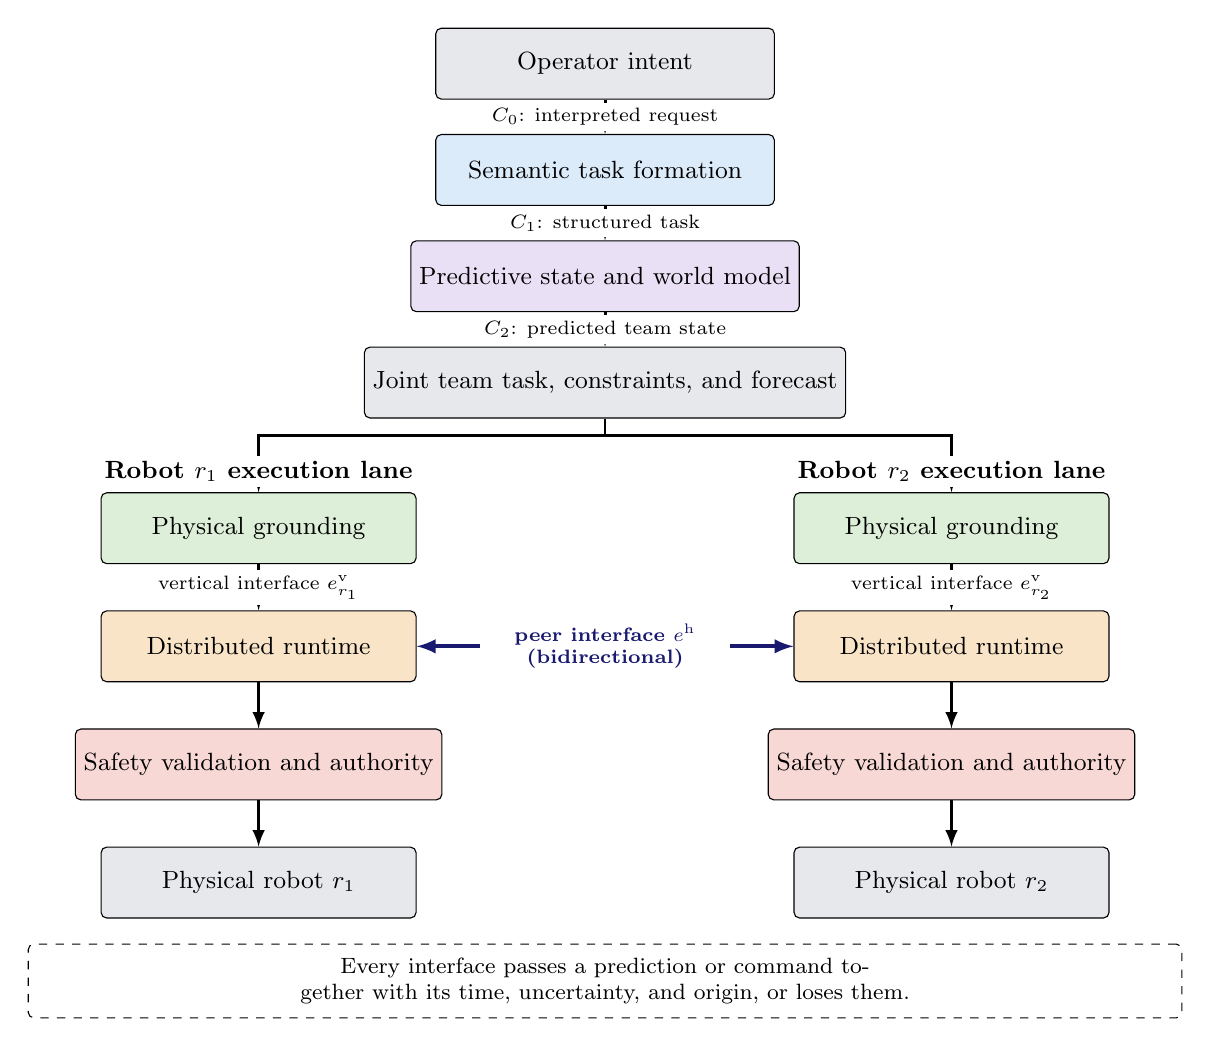
\begin{tikzpicture}[x=1cm,y=1cm]
    % Shared command-formulation path.  All arrows point downward.
    \node[pipeline,fill=RealityGray] (human) at (0,0)
      {Operator intent};
    \node[pipeline,fill=SemanticBlue] (semantic) at (0,-1.35)
      {Semantic task formation};
    \node[pipeline,fill=WorldPurple] (world) at (0,-2.70)
      {Predictive state and world model};
    \node[pipeline,fill=RealityGray] (team) at (0,-4.05)
      {Joint team task, constraints, and forecast};

    \draw[flow] (human.south) -- node[edgelabel]
      {$C_0$: interpreted request} (semantic.north);
    \draw[flow] (semantic.south) -- node[edgelabel]
      {$C_1$: structured task} (world.north);
    \draw[flow] (world.south) -- node[edgelabel]
      {$C_2$: predicted team state} (team.north);

    % Two parallel robot-execution lanes.
    \node[robotstage,fill=PhysicsGreen] (ground1) at (-4.40,-5.90)
      {Physical grounding};
    \node[robotstage,fill=PhysicsGreen] (ground2) at (4.40,-5.90)
      {Physical grounding};
    \node[robotstage,fill=RuntimeOrange] (runtime1) at (-4.40,-7.40)
      {Distributed runtime};
    \node[robotstage,fill=RuntimeOrange] (runtime2) at (4.40,-7.40)
      {Distributed runtime};
    \node[robotstage,fill=SafetyRed] (safety1) at (-4.40,-8.90)
      {Safety validation and authority};
    \node[robotstage,fill=SafetyRed] (safety2) at (4.40,-8.90)
      {Safety validation and authority};
    \node[robotstage,fill=RealityGray] (robot1) at (-4.40,-10.40)
      {Physical robot $r_1$};
    \node[robotstage,fill=RealityGray] (robot2) at (4.40,-10.40)
      {Physical robot $r_2$};

    % The joint plan branches into the two robot lanes.
    \coordinate (split) at (0,-4.72);
    \draw[line width=0.9pt] (team.south) -- (split);
    \draw[branch] (split) -| (ground1.north);
    \draw[branch] (split) -| (ground2.north);

    % Draw lane headings after the branches so the white backgrounds mask lines.
    \node[font=\small\bfseries,fill=white,inner xsep=4pt,inner ysep=2pt]
      at (-4.40,-5.18) {Robot $r_1$ execution lane};
    \node[font=\small\bfseries,fill=white,inner xsep=4pt,inner ysep=2pt]
      at (4.40,-5.18) {Robot $r_2$ execution lane};

    \draw[flow] (ground1.south) -- node[edgelabel]
      {vertical interface $e^{\mathrm v}_{r_1}$} (runtime1.north);
    \draw[flow] (runtime1.south) -- (safety1.north);
    \draw[flow] (safety1.south) -- (robot1.north);

    \draw[flow] (ground2.south) -- node[edgelabel]
      {vertical interface $e^{\mathrm v}_{r_2}$} (runtime2.north);
    \draw[flow] (runtime2.south) -- (safety2.north);
    \draw[flow] (safety2.south) -- (robot2.north);

    % Only this edge is bidirectional: peer state and coordination evidence.
    \draw[peer] (runtime1.east) -- node[edgelabel,font=\scriptsize\bfseries,
      text=MidnightBlue,text width=29mm]
      {peer interface $e^{\mathrm h}$\\(bidirectional)} (runtime2.west);

    \node[obligation,fill=white] at (0,-11.65)
      {Every interface passes a prediction or command together with its time,
       uncertainty, and origin, or loses them.};
  \end{tikzpicture}
  \caption{Multi-robot command path.  Downward arrows are producer--consumer
  transfers; the double-headed horizontal edge exchanges peer state between
  robots.}
  \label{fig:systems-pipeline}
\end{figure}


Every layer makes a claim about its output under assumptions about its input,
whether or not the claim is written down.  The notes therefore treat each
producer--consumer interface as a contract.  \Cref{sec:layers} surveys the
learned components along the path, \cref{sec:contracts} collects the contract
techniques that already exist for robots, and \cref{sec:edge-contracts} sketches
what a contract on a single edge of the path would have to contain.

Three questions guide the notes:
\begin{enumerate}
  \item Where along the command path should a prediction be computed: on board,
    on a peer, or on shared infrastructure?
  \item What must accompany a prediction so that the component that consumes it
    can tell whether it is still valid?
  \item How does a wrong or late prediction propagate through planning,
    communication, and safety layers?
\end{enumerate}
